\section{Motivation}
Rapid advances in high-throughput omics technologies have made it possible to simultaneously study thousands of DNA, RNA, proteins and other molecules to get a detailed and systemic look into the inner workings on the cell. This has enabled large-scale whole-genome and whole-transcriptome association studies that have helped identify thousands of genetic risk factors and molecular mechanisms implicated in diseases. Precision medicine has also emerged as a promising new approach to patient care, using molecular profiling to guide treatment. However, while precision medicine has shown great promise already, especially in cancer therapy \cite{Kato2017}, translational success is still limited \cite{Ginsburg2018}.

Molecular profiling data is both complex and inherently noisy, making it difficult to distinguish molecular changes that cause a disease from changes that are caused by it.
One of the ways researchers have attempted to tackle the complexity of molecular profiling data is to incorporate secondary information, for instance in the form of protein-protein interaction networks, biological pathways and ontological information. This has enabled integrative analyses such as \emph{de novo} network enrichment, combining sequence and network information for homology detection, and gene set enrichment analysis to name a few.
However, current experimental techniques for detecting molecular interactions are error-prone and suffer from technical biases. Furthermore, biological knowledge bases such as BioGRID \cite{Stark2006} and Gene Ontology \cite{Ashburner2000} are constructed by manually curating publications and are, as a result of that, limited by our current biological knowledge and subject to research bias. These biases can lead to misleading results, and it is thus important to critically assess the quality of available biological databases and investigate how accurately they portray \emph{in vivo} cell biology. Genomic structural variants, such as copy number variations, also pose an additional problem when used in association studies since they are not defined as distinct entities the way genes and SNPs are. Additional methodology is thus necessary to discretize structural variants in a way that enables statistical analysis.

In order to effectively utilize the wealth of information hiding in molecular profiling data, sophisticated methods and critical assessments of their quality are necessary. The manuscripts presented in this thesis all attempt to address these issues with respect to different omics data types, including gene expression, genetic variants, copy number variants, molecular interactions or a combination thereof. In the following sections, I provide a general introduction to the concepts and techniques underlying these manuscripts.

\section{The central dogma of molecular biology}
The central dogma of molecular biology formulates the basic process by which genetic information flows from DNA to RNA and into a functional product. The dogma, as it was initially stated by Francis Crick in 1957 \cite{Cobb2017}, hypothesized that when genetic information is transferred into protein, it cannot escape. More than half a century later, our knowledge on genetic information has evolved significantly, but Crick's 1957 lecture was so influential, that \enquote{central dogma} is now colloquially used to denote the general exchange of sequence information in the cell.

The relationship between DNA, RNA and proteins is highly complex and varies between eukaryotes and prokaryotes. However, the primary exchange of genetic information is maintained through three mechanisms: replication, transcription and translation (Figure~\ref{fig:centraldogma}).
DNA \emph{replication} is the process by which DNA is copied during cell division. During replication, the two complementary DNA strands are separated by DNA helicase, producing a replication fork. Each strand acts as a template for building a new two-stranded DNA molecule by DNA polymerase proteins.
During \emph{transcription}, a DNA transcription unit is copied into an RNA molecule. A transcription unit consists of a coding sequence and a number of regulatory elements such as a promoter. Transcription is initiated by RNA polymerase together with one or more transcription factors binding to the promoter. RNA polymerase then separates the DNA strands to form a transcription bubble and adds RNA nucleotides to the template strand to produce an RNA complement\footnote{In the RNA complement uracil nucleotides occur where thymine would have appeared in the DNA complement.}. In eukaryotes, the produced pre-RNA undergoes further processing, including splicing out introns, in order to produce mature RNA (mRNA).
During \emph{translation}, the mRNA is used as a template for synthesizing a polypeptide. A ribosome moves along the mRNA strand reading nucleotide triplets. Starting at the start codon, a peptide chain is built from amino acids matching the triplet sequence until a stop codon is encountered. As it is being assembled, the protein (polypeptide) will fold into a three-dimensional structure determining its function.
%
\begin{figure}
    \centering
    
\includegraphics[width=10cm]{figures/centraldogma.pdf}
    \caption{The central dogma of biology.}
    \label{fig:centraldogma}
\end{figure}

By now, we understand that the central dogma provides a highly simplified view of gene expression as many other processes play a role in genetic regulation. Early on it was suggested that genetic information is also exchanged from RNA to DNA through reverse transcription, and that replication of RNA also occurs \cite{Crick1970}. Epigenetic changes such as DNA methylation and histone modifications can also significantly affect gene expression \cite{Egger2004}. Furthermore, not all transcription units are translated into proteins; some instead code for regulatory non-coding RNAs such as miRNAs \cite{Robinson2009}. Despite this, the central dogma is still at the core of bioinformatics research, and studying cells at the DNA, RNA and protein levels has been fundamental to the elucidation of cellular function.
\todo[inline]{This last section could be much better. Especially last sentence.}

\section{Molecular profiling}
Advances in modern biotechnology have enabled the large-scale study of cells at the molecular level. This has given rise to a broad range of so-called omics studies aiming to study cells as a whole by identifying and quantifying their constituent molecules. Prominent omics studies include genomics, transcriptomics and proteomics, studying cells at the DNA, RNA and protein level, respectively. The following subsections provide an overview of the omics technologies utilized in this thesis.

\subsection{Genomics}
Genomics is the study of genomes, the complete set of DNA for an organism. Early genomics research focused on sequencing the complete genomes. The first complete genome to be published was the \emph{Haemophilus influenzae} bacteria in 1995 \cite{Fleischmann1995}, with the first eukaryotic genome, \emph{Saccharomyces cerevisiae} (or brewer's yeast), being published the following year \cite{Goffeau1996}. However, it would be another 12 years before a comprehensive human genome was published by the Human Genome Project \cite{Venter2001,Genome2004}.

Advances in high-throughput microarray and sequencing technology has rapidly reduced the cost and time of sequencing, making it possible to study the genomes of a large number of individuals \cite{Bumgarner2013,Reuter2015}. Although the human genome consists of 3.2 billion base pairs, a typical genome only differs from the reference genome in 4--5 million sites (0.1--0.2\%), and most individual variants are single-nucleotide polymorphisms (SNPs)\footnote{A substitution of a single nucleotide that occurs in a sizable fraction of the population, typically at least 1\% of the population.} \cite{genomes1k2015}.
% About SNP arrays: https://academic.oup.com/nar/article/37/13/4181/1071175 \cite{LaFramboise2009}
SNP arrays are a type of DNA microarray designed to specifically target SNPs for genotyping. SNP arrays have enabled large-scale genome-wide association studies (GWAS; Section~\ref{sec:gwas}) in which thousands of individual genomes are tested to find single-nucleotide variants associated with a trait. Modern arrays can detect more than \num{900000} SNPs \footnote{The Illumina Genome-Wide Human SNP Array 6.0 has 1.8 million markers of which \num{906600} detect SNPs (\url{https://www.thermofisher.com/order/catalog/product/9011500}).}.

Genome-wide association studies have been instrumental to discovering a large number of disease-associated genetic variants, but for complex traits the known variants together still only explain a fraction of the total heritability. Part of this \enquote{missing heritability} problem may stem from rare variants not detected by SNP arrays \cite{Manolio2009,Lee2014}. With next-generation sequencing, DNA sequencing has emerged as a promising alternative to array-based techniques. Whole-genome sequencing (WGS) avoids the bias from probe selection and is able to detect rare variants. Exome sequencing has also been developed as a more efficient and cheaper alternative to WGS when focusing specifically on protein-coding DNA \cite{Suwinski2019}. The UK Biobank is currently in the process of sequencing whole genomes of \num{50000} participants and exomes of half a million participants\footnote{\url{https://www.ukbiobank.ac.uk/scientists-3/genetic-data}} and the Genomic Data Commons current provides whole exome sequencing data for more than \num{12000} cancer patients \cite{Gao2019}.

\subsection{Copy-number variations}
Copy number variants (CVS) are structural variations where a large segment (e.g. greater than 1 kilobases) of the genome is duplicated or deleted \cite{Redon2006}. Although a typical genome contains relatively few CNVs, they cover a large part of the genome (\sim{}20 million bases) \cite{genomes1k2015}. Microarray-based comparative genomic hybridization (aCGH) is widely used for detecting CNVs between a sample and a reference (e.g. tumor vs. healthy tissue). While aCGH is accurate and cost effective, it is not able to detect balanced rearrangements such as inversions\footnote{When a segment of a chromosome is reversed from end to end.} and is not suited for detecting short CNVs due to lack of resolution \cite{Duan2013}. Whole-genome sequencing can also be used to detect CNVs (see \citeauthor{Zhang2019} \cite{Zhang2019} for a recent review of methods). WGS-based methods are able to detect variants not detected by aCGH and was found to be at least as sensitive in a recent benchmark \cite{Gross2018}.

CNVs have been found to be associated with gene expression levels, suggesting they have a regulatory influence \cite{Stranger2007,Gamazon2015}, and copy number changes have been implicated in a wide range of disorders \cite{McCarroll2007,Girirajan2011}. CNVs are frequently studied in cancer since somatic genomic alterations are common in tumors \cite{Zack2013}. Large CNVs in tumors have been associated with improved response to chemotherapy as a result of defective DNA repair and, based on that, several metrics have been proposed for predicting treatment outcome from genomic scars \cite{Abkevich2012,Birkbak2012,Popova2012,Marquard2015}.

\subsection{Transcriptomics}
Transcriptomics is the study of transcriptomes, the total set of RNA molecules present in a cell. Whereas genomics analysis looks at what the cell is able to do, gene expression analysis tells us what the cell is \emph{currently} doing. Although measuring the actual abundance of proteins would give a more direct estimate of protein activity, proteomics analysis is complex, in part, because as many as 100 different proteins can be produced from a single gene due to alternative splicing, SNPs and post-translational modifications \cite{Ponomarenko2016}, making gene expression an attractive proxy for protein activity. However, some studies have reported the correlation between mRNA and protein abundance to be rather modest, which suggests gene expression may be misleading for measuring protein activity under some conditions \cite{Rogers2008,Maier2009,Schwanhaeusser2011,Ghazalpour2011}.

Like in genomics, microarrays have, until recently, dominated gene expression analysis, but in recent years, RNA-seq (or whole-transcriptome shotgun sequencing) has become the primary method for whole-transcriptome analysis as a result of rapidly decreasing sequencing costs and improved computational methods \cite{Wang2018}. Large amounts of gene expression data is already publicly available in data repositories such as the Gene Expression Omnibus \cite{Barrett2012} and ArrayExpress \cite{Athar2018}, and through large-scale research initiatives like the Genomic Data Commons \cite{Gao2019}.

One of the main applications of gene expression data is differential expression analysis, in which the expression level of each gene is tested for association with a phenotype (e.g. disease status) using an appropriate test statistic. While many early studies have used two-sample hypothesis tests (e.g. Students \textit{t}-test, Wilcoxon signed-rank test) modern methods for gene expression analysis, such as limma \cite{Ritchie2015} or DESeq2 \cite{Love2014}, are based on linear models. Gene expression data is also used in unsupervised analysis to discover genes that are functionally related  \cite{Stuart2003} or to separate patients into clinically relevant subgroups \cite{Perou2000,Parker2009,Wilkerson2010,Bailey2016}.

\todo[inline]{This section is weak. Try to improve. Maybe more examples in last part?}

\section{Genome-wide association studies}
% Figur med PC <-> geography: https://www.nature.com/articles/nature07331
\label{sec:gwas}
A genome-wide association study (GWAS) is a type of statistical study in which a genome-wide set of genetic variants are tested for association with a phenotype. GWASs are most commonly applied to SNPs, but can also be applied to other types of genetic variants such as CNVs. A typical GWAS setup includes a case-control setup where SNPs are tested for association with a disease, but the outcome can also be a clinical variable such as body mass index or blood pressure.
In the study, each SNP is tested individually for association using a test statistic (e.g. Fisher's exact test) or using regression analysis. Regression-based analysis is most commonly used as it allows for the inclusion of additional variables such as sex and age, which generally needs to be adjusted for.
Whole-genome GWAS exploit linkage disequilibrium to cover most of the genome by genotyping tag SNPs. Because of this, the reported SNPs are likely not the causal variants, and subsequent fine-mapping is required to identify the actual causal variant(s) \cite{Spain2015}. Genotype imputation methods have also been developed for imputing the genotype of SNPs not directly genotyped using whole-genome sequence data from a reference population \cite{Browning2007,Li2009,Howie2009}.

A major source of confounding bias in genetic studies is population stratification. Differences in allele frequencies between subpopulations in a cohort can lead to spurious associations that arise due to population structure even if the variant is not associated with the outcome. Correction for population structure is commonly done using principal component analysis, as introduced in EIGENSTRAT \cite{Price2006}, or using a linear mixed-model approach e.g. EMMA/GEMMA \cite{Kang2008,Zhou2012}.

Due to the large number of SNPs under consideration, GWASs are subjected to a strong multiple testing burden, traditionally addressed using Bonferroni correction resulting in a \textit{p}-value cutoff around $5 \times 10^{-8}$. One way this problem has been addressed is to perform association tests at the gene or gene set (pathway) level to significantly reduce the number of tested hypotheses. Prominent examples of gene and gene set level enrichment tests include PLINK \cite{Chang2015}, MAGMA \cite{Leeuw2015}, MAGENTA \cite{Segre2010} and GSEA-SNP \cite{Holden2008}. These methods are closely related to functional class scoring methods (Section~\ref{sec:genesetenrichment}) used in gene expression analysis.
\todo[inline]{Additive, dominant, recessive?}

\section{Molecular networks}
Understanding the vast complexity of living cells requires not only an understanding of the individual biological entities but also how they interact. It is increasingly clear that virtually all biological processes are carried out not by a single agent, but by a complex interaction between various entities such as proteins, RNA, DNA, metabolites and environmental factors. The study of cellular interactions or relationships naturally lends itself to be modeled as a network. As a result of this, network biology has become a key area of bioinformatics research, focusing on constructing and analyzing networks of a wide range of relationship types, including protein-protein interactions, transcriptional regulatory interactions, drug-target associations and signaling pathways.

\subsection{Network modeling}
Biological networks are most commonly modeled as graphs. A graph is described by a set of vertices (or nodes) and a set of edges connecting pairs of nodes. Graphs can be defined in a multitude of ways depending on the context they are used in (Figure~\ref{fig:graphtypes}).

An \emph{undirected graph} is a pair $G=(V,E)$ where $V$ is a set of vertices and $E$ is a set of two-sets describing edges. This definition implies that edges do not have directionality. Undirected graphs are commonly used to model protein-protein interactions where the direction of effect is generally not known due to experimental limitations \cite{Vinayagam2011}. Undirected graphs are also referred to as \emph{simple} graphs to distinguish them from \emph{multigraphs} in which $E$ is a multiset thus allowing for parallel edges and self-loops.

A \emph{directed graph} is a pair $G=(V,E)$ where $V$ is a set of vertices and $E$ is a set of ordered pairs. Directed graphs are used to model relationships with an inherent directionality, such as signaling pathways and metabolic pathways. A \emph{directed acyclic graph} (DAG) is a graph with no directed cycles. A directed graph is a DAG if and only if it has a topological ordering. Biological ontologies, such as the Gene Ontology \cite{GeneOntology2018}, are naturally represented as DAGs due to their hierarchical organization.

A \emph{bipartite graph} is a triplet $G=(U,V,E)$ where $U$ and $V$ are disjoint sets of vertices and $E$ is a set of edges connecting a vertex in $U$ to a vertex in $V$. Bipartite graphs are used for modeling networks where relationships map from one class of entities to another such as drug-target interactions and transcription factor-gene regulatory interactions.

A \emph{weighted graph} is a graph where each edge is assigned a numerical weight. Weighted graphs are commonly used to model networks of pairwise similarities such as gene co-expression, patient similarity and disease comorbidity networks. Edge weights may also be used to include confidence scores of interactions to factor in uncertainty in the detection method.

\noindent Other graph definitions such as \emph{hypergraphs} and \emph{mixed} graphs also exist, but will not be discussed in this thesis.
%
\begin{figure}
    \centering
    \subbottom[Undirected]{\includegraphics[height=4.5cm]{figures/graph_ex_undir.tikz}}
    \hfill
    \subbottom[Directed]{\includegraphics[height=4.5cm]{figures/graph_ex_dir.tikz}}
    \hfill
    \subbottom[Bipartite]{\includegraphics[height=4.5cm]{figures/graph_ex_bipart.tikz}}
    \hfill
    \subbottom[Weighted]{\includegraphics[height=4.5cm]{figures/graph_ex_weighted.tikz}}
    \caption{Overview of different graph definitions.}
    \label{fig:graphtypes}
\end{figure}

\subsection{Protein-protein interaction networks}
Most cellular processes are not maintained by a single protein but, rather, by complexes of multiple proteins linked by protein-protein interactions (PPIs), interactions between proteins established through highly specific physical contacts. Consequently, identifying the complex network PPIs has become a key problem in bioinformatics.

A wide range of experimental methods have been developed for PPI detection.
Tandem affinity purification coupled to mass spectrometry (TAP-MS) is a widely used \emph{in vitro} method for high-throughput PPI detection. TAP-MS is able to detect both protein pairwise interactions and multi-protein complexes with high sensitivity. However, it is only reliable for detecting stable interactions as transient (short-lived) interactions will generally be missed due to the tandem purification steps. Yeast two-hybrid (Y2H) screening is another high-throughput method that directly detects PPIs between protein pairs \emph{in vivo}. Y2H screening is comparatively simple and inexpensive to run, and is able to detect transient interactions. However, it suffers from a high false positive positive rate. Affinity purification methods may be biased in favor of high-abundance proteins, while this does not appear to be the case for yeast two-hybrid \cite{Ivanic2009}.
Co-immunoprecipitation is generally considered the gold standard for detecting PPIs. It requires selecting an antibody that targets a specific protein believed to interact in a complex, making it infeasible for screening. It is, however, a highly accurate method for confirming interactions reported by high-throughput techniques \cite{Berggard2007,Rao2014}. Protein-protein interactions have also been predicted \emph{in silico} using protein sequence, three-dimensional structure, co-expression, network topology and Gene Ontology annotations \cite{Elefsinioti2011, Zhang2012, Kotlyar2014}, among other features.

For two decades, protein-protein interactions have been curated in large, publicly available databases. The first PPI database DIP (Database of Interacting Proteins) was published in 1999 \cite{Xenarios2000}. Current PPI databases such as BioGRID \cite{Stark2006} and STRING \cite{Szklarczyk2014} contain hundreds of thousands of interactions across a multitude of species derived from literature and \emph{in silico} prediction. These databases enable the construction of a network comprising of the entire set of interactions, commonly referred to as an \emph{interactome}. Protein-protein interaction networks are generally modeled as simple graphs (Figure~\ref{fig:ppinetwork}), as they lack direction and edge weight, although some protein interaction databases do include a form of interaction score \cite{Szklarczyk2014,Alanis-Lobato2016}. Interactomes have become an important resource in bioinformatics research as they provide a structured overview of which genes/proteins are interacting or otherwise functionally related. For instance, interactomes are used to predict orthologs through network alignment analysis (Section~\ref{sec:networkalignment}) and to discover disease gene modules and biomarkers (Section~\ref{sec:diseasemodule}).
%
\begin{figure}
    \centering
    \includegraphics[width=11cm]{figures/ppi_biogrid_kk.jpg}
    \caption{The BioGRID protein-protein interaction network drawn as a simple graph using the Kamada \& Kawai layouting algorithm. Node size is proportional to log10 of the node degree.}
    \label{fig:ppinetwork}
\end{figure}

Biological networks have frequently been claimed to resemble a scale-free network, that is, a network whose degree distribution resembles a power law \cite{Jeong2001,Barabasi2004,Goh2002}. This claim is, however, controversial and many authors have argued the scale-free properties are a result of research bias or that other graph models are more appropriate \cite{Przulj2004,Khanin2006,Przulj2007,Lima-Mendez2009,Broido2019}. Early studies of PPI networks identified that high-degree proteins were generally more important for cell survival \cite{Jeong2001,Hahn2004}. However, later this essentiality-connectivity rule was brought into question by subsequent studies. Affinity purification methods may be biased in favor of essential proteins since they are more abundant \cite{Ivanic2009}. Node degree is also highly correlated with number of publications describing a protein, suggesting essential proteins are hubs partly because they are highly researched \cite{Rolland2014}.

\subsection{Transcriptional regulatory networks}
Transcriptional regulation is a vital process that ensures the right amount of RNA is produced at the right time in order to control gene activity in the cell. Transcriptional regulation functions very differently between prokaryotes and eukaryotes, and prokaryotic regulatory mechanisms are overall more well-understood due to being less complex and easier to investigate. Transcription in prokaryotes is mainly regulated is by means of transcription factors (TFs); proteins that bind to specific DNA sequences to regulate the transcription of downstream genes.

Transcriptional regulation has been heavily researched in \emph{E. coli} (in particular in the K-12 strain) with thousands of TF-gene interactions now reported in databases like RegulonDB \cite{Santos-Zavaleta2018} and EcoCyc \cite{Keseler2016}. Many experimental techniques have been developed for high-throughput detection of regulatory interactions, including chromatin immunoprecipitation technology (ChIP-chip or ChIP-seq), protein binding microarrays and systematic evaluation of ligands by exponential enrichment (SELEX) \cite{Geertz2010,Weiss2013}.
Similar to protein-protein interactions, TF-gene interactions can be used to construct a transcriptional regulatory network, in order to study the complex system of interactions regulating the cell.
Considerable effort has also been put into predicting regulatory interactions from genome-wide gene expression data; most notably this problem was the focus of four separate DREAM challenges \cite{Stolovitzky2009,Marbach2010,Prill2010,Marbach2012}.

\subsection{Biological pathway databases}
A biological pathway is a set of interactions between molecules that work together in order to carry out a certain task in the cell. Examples of common pathway types include metabolism, cell signaling and genetic regulation. Pathways differ from the previously described networks in that they don't model one specific type of interaction but rather a combination of various molecular interactions and reactions. Thus, pathways cannot simply be constructed from a single experimental technique but are instead constructed piece by piece over time as a curated, collaborative effort integrating multiple publications and databases \cite{Pico2008}. The first major pathway database to be published was KEGG in 1995 \cite{Kanehisa2000}, followed by HPRD \cite{Peri2003}, Reactome \cite{Joshi-Tope2004}, PANTHER \cite{Mi2009} and the community-driven database WikiPathways \cite{Pico2008}.
These pathways provide visual overviews of each pathway in the form of pathway diagrams (Figure~\ref{fig:reactome_hedgehog}) as well as standardized human-readable formats such as BioPAX \cite{Demir2010} and SBML \cite{Hucka2018} to enable computational analysis and data sharing.
%
\begin{figure}
    \centering
    \includegraphics[width=\linewidth]{figures/reactome_hedgehog.png}
    \caption{Pathway diagram of the \enquote{Signaling by Hedgehog} pathway in Reactome (\url{https://reactome.org/PathwayBrowser/\#/R-HSA-5358351}).}
    \label{fig:reactome_hedgehog}
\end{figure}

\subsection{Biological ontologies}
In informatics, an ontology is a formal representation of the entities in a specific domain, the relations between the entities and their properties. Ontologies develop a controlled vocabulary for describing concepts without the ambiguity inherent in natural languages. Ontologies most commonly describe objects in terms of \enquote{is a}-relations, but may include other types of relations depending on the domain. Similar to biological pathway databases, ontologies are generally created through manual curation of literature and evolve over time as domain knowledge accumulates.

The most prominent biological ontology is the Gene Ontology (GO) \cite{GeneOntology2018}, an ontology describing genes and gene products across multiple species. GO describes the function and structure of the cell as a hierarchy of terms covering three domains: cellular component, molecular function and biological process. For instance, from the cellular component ontology, we can infer that the Golgi apparatus is \emph{part of} the endomembrane system and that the Golgi apparatus \emph{is an} organelle (Figure~\ref{fig:ontologies}a). Genes and gene products are described by annotating them with terms from the ontology, in order to provide a detailed description of their function and subcellular localization.
Other ontologies, such as the Disease Ontology \cite{Kibbe2014}, provide a formal description of human disease (Figure~\ref{fig:ontologies}b). Ontologies are generally made available in standardized, machine-readable formats such as the Open Biological and Biomedical Ontology format (OBO) and the Web Ontology Language (OWL). This has enabled ontology-based computational analyses such as measuring the semantic similarity between genes based on their GO terms annotations \cite{Mazandu2016}.
%
\begin{figure}
    \centering
    \subbottom[]{\includegraphics[height=7.8cm]{figures/go_golgi.pdf}}
    \hfill
    \subbottom[]{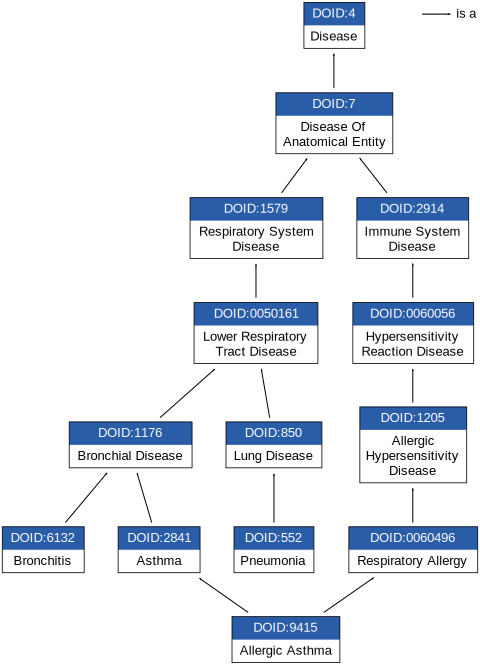
\includegraphics[height=7.8cm]{figures/do_lung.pdf}}
    \caption{Examples of ontology ancestors charts. (a) Ancestor chart for the Gene Ontology term \enquote{Golgi apparatus} (GO:0005794). (b) Subhierarchy from Disease Ontology describing select respiratory diseases.}
    \label{fig:ontologies}
\end{figure}

\subsection{Gene set and pathway enrichment analysis}
\label{sec:genesetenrichment}
Differential expression analysis has become a core part of biomedical research for identifying genes and proteins where a change in expression is associated with a change in phenotype. However, the results are often difficult to interpret as-is. Pathway databases and ontologies like KEGG and Gene Ontology provide detailed functional information about genes and gene products and are thus a valuable reference for downstream analysis following differential expression analysis. \emph{Pathway enrichment} has been proposed for functional annotation of gene expression results, by identifying pathways that are significantly enriched. Pathway enrichment methods can roughly be separated into three types:

\paragraph{Gene set overrepresentation test (GSO)}
Early gene set enrichment methods would test whether a set of candidate genes were statistically overrepresented in the reference gene sets. The set of candidates would generally comprise of genes that met some differential expression significance criterion (e.g. a false discovery rate of 5\%). For each reference gene set, the significance of overrepresentation is computed as the probability of observing an equally large or greater overlap between the candidate and reference gene sets if candidate genes were selected randomly. This test is commonly performed based on the hypergeometric, binomial or chi-squared distribution \cite{Huang2008}.
While GSO is simple to compute and does not rely on permutation tests, it suffers from some major drawbacks. Most importantly, because the inclusion criterion is binary, all candidate genes are considered equally important even if they have vastly different fold changes, and the direction of effect (i.e. over- or underexpressed) is ignored.

\paragraph{Functional class scoring (FCS)}
Functional class scoring methods use the entire set of gene-level statistics to identify enriched gene sets. Commonly used test statistics include the fold-change, $t$-statistic, regression coefficient and correlation coefficient \cite{Ackermann2009}. The gene-level statistics are then aggregated into a gene set-level statistic. Finally, the significance of each gene set is estimated using permutation tests. The permutation scheme depends on whether the null hypothesis is self-contained or competitive: self-contained tests compare each gene set with itself under no association (i.e. permuted phenotype). A competitive test instead compares a gene set to all other genes not in the set. In other words, the self-contained null hypothesis states that \emph{no genes in the set are differentially expressed} while the competitive null hypothesis states that \emph{genes in the set are no more differentially expressed than genes not in the set}.

One of the earliest and most widely-used FCS methods is the Gene Set Enrichment Analysis (GSEA) \cite{Subramanian2005}. GSEA uses a Kolmogorov-Smirnov-like statistic to calculate how much genes in the gene set are overrepresented at the extremes of the gene-level statistic (i.e. over- or underexpressed). Despite its ubiquity, GSEA is generally outperformed by other methods using simple gene set statistics such as mean or sum \cite{Ackermann2009,Hung2011,Mathur2018}. FCS methods overcome the limits of needing a significance cutoff inherent to GSO methods. By utilizing the entire set of gene-level statistics, they are also able to discover enriched gene sets even if no single gene in the set is significantly differentially expressed.

\paragraph{Pathway topology-based methods (PT)}
Pathway databases provide a detailed view of not just the genes participating in a pathway, but also the way they interact. GSO and FCS methods consider only which genes are part of a pathway---not how they are connected. PT methods generally work similarly to GSO and FCS methods, but incorporate additional topological information when computing the gene-level or gene set-level statistics.
I refer to recent evaluations by \citeauthor{Bayerlova2015} \cite{Bayerlova2015} and \citeauthor{Ihnatova2018} \cite{Ihnatova2018} for a detailed overview.

\subsection{\emph{De novo} network enrichment}
\label{sec:diseasemodule}
% Cells are believed to inherently modular:
%   https://doi.org/10.1126/science.1089072
%   https://doi.org/10.1016/j.cell.2005.04.020
% DNE reviews:
% - https://www.ncbi.nlm.nih.gov/pmc/articles/PMC5445589/
% - https://bmcbioinformatics.biomedcentral.com/articles/10.1186/s12859-017-1567-2
Pathway enrichment methods have been very useful for discovering mechanisms affected by expression changes. However, they are ultimately limited by how complete the underlying knowledge base is. If a disease or intervention affects a pathway that has yet to be discovered, it will not be reported by any enrichment method regardless of methodology. \emph{De novo network enrichment} methods instead aim to discover enriched pathways \emph{de novo} in a global interaction network. Given a network, e.g. a PPI network, and a gene expression data set (or some gene-level test statistic) \emph{de novo} network enrichment methods aim to discover subnetworks that exhibit statistically significant enrichment.
Existing methods can roughly be separated into four categories: aggregate score optimization, network propagation, module cover and clustering-based \cite{Batra2017}.

\paragraph{Aggregate score optimization (ASO)} These methods are analogous to functional class scoring (Section~\ref{sec:genesetenrichment}) except gene sets are not defined \emph{a priori}. Each gene is first assigned some score, typically derived from a case-control experiment. These scores can be a test statistic, \textit{p}-value, fold-change etc. ASO methods then aim to find a connected subnetwork with maximum aggregated score. Depending on the problem formulation, finding such a subnetwork is generally equivalent to the maximum weight connected subgraph problem or the maximum weight connected $k$-induced subgraph problem, both of which are NP-hard \cite{Johnson1985,Ideker2002}. This type of analysis was first introduced by \citeauthor{Ideker2002} in jActiveModules, where they used a simulated annealing algorithm to find a subnetwork with maximum aggregated z-score \cite{Ideker2002}. Other prominent methods using similar methodology include BioNet \cite{Beisser2010} and PinnacleZ \cite{Chuang2007}. Some authors have also proposed assigning scores to edges instead, based on co-expression \cite{Guo2007} or combining gene \textit{p}-values \cite{Cabusora2005}.

\paragraph{Network propagation (NP)} Methods based on network propagation work by first assigning a score (or \enquote{heat}) to each node in the network and then simulating how that signal propagates through the network over time such that the signal accumulates in signal-rich subnetworks. Most NP methods are based on either heat diffusion \cite{Vandin2012,Paull2013}, random walks \cite{Erten2011,Komurov2012} or network expansion from seed genes \cite{Breitling2004,Nacu2007}. Unlike ASO methods, NP does not extract a connected subnetwork, but instead reprioritizes the genes using the network. However, by simulating network flow, NP methods utilize the network topology beyond just connectivity. Besides differential analysis, NP methods are also prominently used in analyzing genetic variants and somatic mutations in cancer \cite{Leiserson2014,Cowen2017,Zhang2018,Carlin2019}.

\paragraph{Module cover (MC)} These methods operate in two steps: first, a set of key genes are selected. Key genes typically comprise of significantly differentially expressed genes, but can also be disease genes known \emph{a priori}. Then a connected subnetwork with high key gene density is extracted under some constraint; typically restricting the total number of genes or the number of non-key genes allowed. Some methods, such as CUSP \cite{Ulitsky2008} and KeyPathwayMiner \cite{Alcaraz2011}, determine differential expression on a per-patient basis and allow exceptions both on the gene and patient level. By decoupling the selection of key genes from the subnetwork extraction, no assumptions are made on the underlying data, and an appropriate statistic can instead be selected depending on the data set.  However, the choice of significance cutoff for genes, as well as the target module size or number of exceptions significantly affect the results \cite{Batra2017} which can make MC methods more difficult to apply and interpret.

\paragraph{Clustering-based} These methods employ clustering techniques in some way, to identify groups of differentially expressed genes that are closely connected and co-expressed. ClustEx clusters genes into modules using hierarchical clustering and then builds connected subnetworks of differentially expressed genes as a separate step \cite{Gu2010}. cMonkey uses bi-clustering to cluster genes into modules based on network topology and phenotype simultaneously \cite{Reiss2006}. \citeauthor{Wu2012} used Markov clustering to cluster genes into disease-specific interaction modules and then used supervised principal component analysis to identify clinically significant modules \cite{Wu2012}.

\subsection{Network alignment}
\label{sec:networkalignment}
Network alignment (NA) is the problem of finding a mapping between the nodes in two or more networks (usually from different species) that identifies nodes or small subnetworks that play similar roles in their respective networks. Research on biological NA has mainly focused on aligning protein-protein interaction networks, that is, mapping proteins across different species. The main motivation for finding such a mapping is that the mapped proteins are expected to be likely orthologs or functionally similar. This may, in turn, aid the transfer of knowledge from a model species to another species such as humans. NA has been used to predict missing interactions by aligning a yeast PPI network to human, to find interacting proteins in yeast mapped to non-interacting proteins in human \cite{Malod-Dognin2015}. NA was also used to predict functional of unannotated proteins in one network based on their mapped proteins in other species \cite{Meng2016}.
%Homology detection has traditionally been based on protein sequence comparison, but network information has been shown to provide complementary information for finding orthologs \cite{Memisevic2010}.

Network alignment approaches can be separated into \emph{local} and \emph{global}. Local network alignment (LNA) methods map small conserved subnetworks across different networks, typically producing a many-to-many mapping (Figure~\ref{fig:networkalignment}a). Global network alignment (GNA) methods instead aim to map (almost) all nodes in one network to another, typically in a one-to-one fashion (Figure~\ref{fig:networkalignment}b). Over time research has shifted to mainly focus on one-to-one global alignment \cite{Faisal2015,Guzzi2017}.
From a computational perspective, the one-to-one global network alignment problem is the problem of finding a mapping that maximizes some objective function. The objective function varies between methods but is meant to capture the overall conservation of interactions across species. Some methods also incorporate other information into the objective function such as sequence similarity. When the objective function is simply the number of conserved edges, the problem is equivalent to the maximum common edge subgraph problem which a generalization of the subgraph isomorphism problem, a known NP-complete problem\footnote{Cook proved the subgraph isomorphism problem is NP-complete by reduction from the 3-SAT problem.} \cite{Cook1971}. Consequently, most definitions of the GNA problem are NP-hard. Due to the intractability of the underlying optimization problem, most methods employ metaheuristics or relaxed integer programming to compute good solutions within a reasonable time \cite{Guzzi2017}.
% Maybe write about inclusion of node similarities like sequence similarity or graphlet degree vectors?
% Maybe write that
%
\begin{figure}
    \centering
    \subbottom[Local alignment]{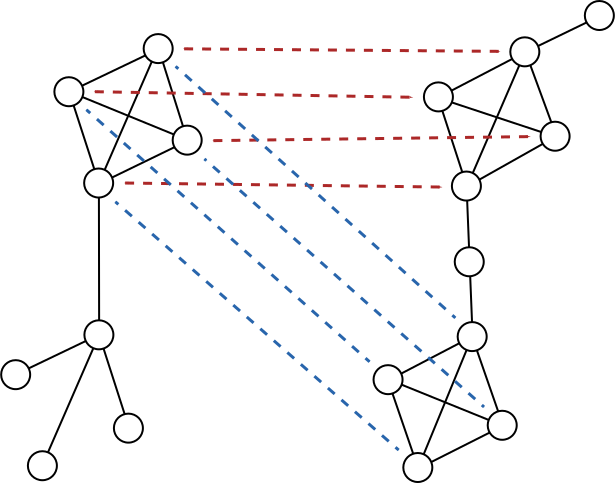
\includegraphics[height=5cm]{figures/local_alignment.pdf}}
    \hfill
    \subbottom[Global alignment]{\includegraphics[height=5cm]{figures/global_alignment.pdf}}
    \caption{Pairwise local and global alignments of two undirected networks. Adapted from \citeauthor{Meng2016} \cite{Meng2016}.}
    \label{fig:networkalignment}
\end{figure}

\section{Decision trees and random decision forests}
Decision tree learning is a non-parametric machine learning method in which a decision tree is grown on a dataset and subsequently used as a predictive model. A decision tree is a tree-like model, similar to a flowchart, wherein each internal node corresponds to a predicate (i.e. a boolean-valued function) on a specific variable, and each leaf node corresponds to a prediction (Figure~\ref{fig:rpart_iris}). Most methods build decision trees in a greedy, top-down fashion: given a set of independent variables and a single dependent variable, the splitting procedure selects the variable-value pair (split rule) that best separates the samples wrt. the dependent variable based on some metric. Samples are then split into two partitions based on this split rule, and the splitting procedure is applied recursively for the two partitions. The recursive partitioning stops when a node is pure, meaning all samples are of the same class, or when no improving split exists. A wide range of decision tree algorithms exist, most notably the seminal models, CART \cite{Breiman1984} and ID3 \cite{Quinlan1986}, and later C4.5 \cite{Quinlan1994}, an extension of ID3.
%\todo[inline]{Maybe write a bit about split rule selection metrics.}
% Different metrics have been proposed for choosing split rules. CART uses the Gini impurity, measuring the

Decision tree learning has several beneficial properties: decision trees can include both numerical and categorical variables. Variable selection is an inherent part of the tree building process. Because split rules for numeric variables are binary (e.g. \enquote{less than}), the tree growing procedure is invariant to monotonic transformation and does not make any assumptions about the distribution of the data (e.g. normality). Finally, the produced decision trees are easy to visualize and interpret. Despite these properties, decision trees are rarely used in practice due to high variance and overall poor predictive performance.

Tin Ho introduced random decision forests in which multiple decision trees are grown using the random subspace method \cite{Ho1995} (also known as feature bagging) and then used as an ensemble learning method. Breiman and Cutler's Random Forests method extended Ho's method to use bootstrap aggregating (or bagging) and furthermore introduced the out-of-bag error for estimating the generalization error and the use of permutation for estimating variable importance \cite{Breiman2001,Breiman2003}.

Using a large ensemble of decision trees trained on different parts of the dataset reduces model variance without increasing bias, and systematic evaluations have shown Random Forest achieves great predictive performance compared to other methods \cite{Caruana2006,Caruana2008}. Decision tree forests are also able to capture variable interactions but their ability to distinguish interaction effects from marginal effects is limited \cite{Lunetta2004,McKinney2006,Wright2016}. Besides classification, Random Forest has also been extended to support regression \cite{Breiman2001}, probability \cite{Malley2012} and survival analysis \cite{Ishwaran2008}.
%
\begin{figure}
    \centering
    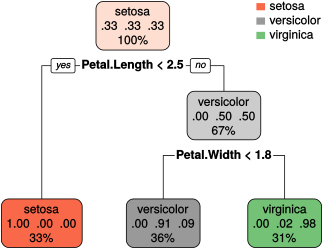
\includegraphics[width=9cm]{figures/rpart_iris.pdf}
    \caption{A classification decision tree classifier trained on the famous Fisher's \emph{Iris} dataset.}
    \label{fig:rpart_iris}
\end{figure}

\clearpage
\section{Hypotheses and aims}
This thesis is presented as a collection of manuscripts related to the development of methods for analyzing complex biomedical data. We identified five main hypotheses and aims that we wanted to focus on.

\paragraph{Aim 1}
The maximum common subgraph problem is a well-known NP-hard problem in graph theory. Despite its ubiquity, there were no tools available for finding good solutions to the MCS problem for large (e.g. interactome size) networks at the inception of this thesis. We aim to develop a new MCS algorithm for large networks that is able to run on a personal computer in a reasonable time. We further aim to make this easily available to researchers by implementing an app for the Cytoscape software platform.

\paragraph{Aim 2}
Genome-wide association studies in single-nucleotide polymorphisms have helped discover thousands of genetic variants associated with human traits and disease. Similarly, copy number variation-based association studies have aided the discovery of important structural variants. However, currently available tools for CNV analysis are limited and hard to use. We aim to develop a new method for CNV-based association studies that is easy to use and enables further analysis beyond testing association.

\paragraph{Aim 3}
Inferring regulatory interactions from gene expression data is a long-standing problem in bioinformatics. Although it has been the focus of several DREAM challenges, even the best methods only perform well on simulated data. We hypothesize that this limited success partly results from a lack of understanding of how regulatory interactions are actually reflected in mRNA levels. We aim to systematically test the assumption that the up- and downregulation of gene coding for transcription factors will result in an interaction-dependent change in the expression of their targets, depending on the type of interaction.

\paragraph{Aim 4}
Random Forest has been shown to be able to discover and utilize interactions between covariates. We hypothesize that decision tree forests are promising for integrating network-structured information since decision trees can naturally be restricted to reflect the network's structure. We aim to explore the use of decision tree forests for integrating biological networks with gene expression data in order to reprioritize genes and discover enriched subnetworks. We will develop a method based on the Random Forests algorithm in which each decision tree induces a connected subnetwork in the interaction network.

\paragraph{Aim 5}
Recent work studying somatic mutations and genetic perturbations has demonstrated that ontologies are promising as an alternative to flat gene sets, allowing the study of accumulated signal at multiple abstraction levels. We hypothesize that using a gene hierarchy to study genetic variants will provide a structured and detailed view of which cellular components and processes are enriched with outcome-associated variants. Furthermore, we hypothesize that the use of a hierarchical model will help filter redundant associations. We aim to implement a gene hierarchy-based method for genome-wide association studies. We further aim to apply this method to find novel associations in a chronic obstructive pulmonary disorder cohort.
